\documentclass{rapport}

\usepackage{lipsum}

\usepackage{gensymb}

\usepackage{float}

\usepackage{graphicx} % Required for inserting images

\title{file title} %title of the file

 

\begin{document}

 

%----------- Report information ---------

 

\logo{src/ua_iut_h_couleur_ecran.png}

\uni{\textbf{IUT Angers}}

\ttitle{Rapport Mini Projet SIN} %title of the file

\name{Shot Timer} % Project Name

\subject{Rapport Shot Timer} % Subject name

\topic{Raport de projet} % Topic name 

\professor{M. Sylvain PEZERIL \\
           M. Benjamin DUTRUCH}

\students{Matéis RAGON} % information related to the students

 

%----------- Init -------------------

\buildmargins % display margins

\buildcover % create the front cover of the document

\toc % creates the table of contents

%------------ Report body ----------------

\section{Rappel du cahier des charges}

Un \textbf{Shot Timer} est un dispositif électronique utilisé principalement dans le cadre du tir sportif ou d’entraînement au tir, que ce soit avec des armes à feu, des armes airsoft. Sa fonction principale est de mesurer les temps liés aux tirs, permettant ainsi aux tireurs d'évaluer leur vitesse, leur efficacité et leurs performances.
\newline
\newline
Ici, nous ne traiterons pas les fonctions d’un Shot Time classique tel que :
\begin{itemize}
    \item L’affichage des statistiques (Split Time\footnote{Split Time : Temps entre deux tirs}  moyen, temps de réaction du premier tir)
    \item La programmation de scénarios
    \item Sauvegarde des sessions de tirs
    \item Démarrage aléatoire de la session de tir
\end{itemize}
\newline
En revanche, nous traiterons les fonctions telles que :
\begin{itemize}
    \item Lancer une session de tir
    \item Arrêter une session de tir s'il n'y a pas de tir pendant 10 s 
    \item Reset le Shot Timer
    \item Comptabiliser les tirs
    \item Afficher des statistiques basiques (meilleur Split Time, temps total, nombre de tirs total)

\end{itemize}


\section{Schéma fonctionnel}

\begin{figure}[h!]

    \centering

    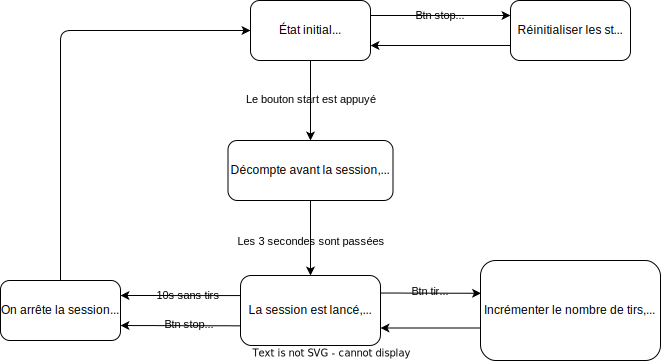
\includegraphics[width=0.8\textwidth]{src/diagram_mini_projet.png}

    \caption{Schéma fonctionnel du Shot Timer}

    \label{fig:functional_diagram}

\end{figure}

Notre schéma fonctionnel est composé de trois grands blocs. Le premier bloc est constitué d'un état initial et d'une réinitialisation des statistiques. Le second bloc gère le décompte avant la session de tir. Et pour finir, le troisième s'occupe de la session en elle-même.

\section{Schéma fonctionnel \textbf{Quartus®}}

\textbf{Quartus®} est un logiciel édité par Intel qui permet de développer sur des cartes telles que la "Altera Cyclone 2 Education Board" qu'on utilise en cours. Ce logiciel permet de développer des programmes sous forme de blocs logiques, et le logiciel compile ensuite les logigrammes en langage VHDL.


\begin{figure}[h!]

    \centering

    \includegraphics[width=0.8\textwidth]{src/seq_n_tirs_part.png}

    \caption{Schéma \textbf{Quartus®} - Séquenceur et compteurs de tirs}

    \label{fig:functional_diagram}

\end{figure}

Sur la figure ci-dessus est mis le séquenceur, le générateur d'horloge ainsi que les compteurs de tir. Il y a deux compteurs, car à l'origine, il est possible de tir jusqu’à 99 fois, cependant à défaut d'avoir assez d'afficheurs sept segments, il a été choisi que l'afficheur des dizaines servirait pour afficher les états du séquenceur.

\begin{figure}[h!]

    \centering

    \includegraphics[width=0.8\textwidth]{src/decompte_part.png}

    \caption{Schéma \textbf{Quartus®} - Décompte avant la session de tir}

    \label{fig:functional_diagram}

\end{figure}

La partie de décompte avant la session de tir est composée d'un compteur, qui est initialisé à la valeur 4. Elle-même mise dans le chargement parallèle avec une constante. Nous avons ensuite un comparateur pour chaque valeur du compteur pour aller à zéro (trois, deux et un). Puis ces comparateurs délivrent un niveau logique haut pour allumer les leds.
\newpage

\begin{figure}[h!]

    \centering

    \includegraphics[width=0.8\textwidth]{src/time_part.png}

    \caption{Schéma \textbf{Quartus®} - Compteurs du temps}

    \label{fig:functional_diagram}

\end{figure}

La partie des compteurs de temps est assez simple puisqu'elle ne contient uniquement des compteurs qui s'enchainent pour former un chronomètre, minutes, secondes et dixième de secondes. Ici, il a été fait le choix de n'afficher que les minutes et secondes, encore une fois par limitation matérielle.

\begin{figure}[h!]

    \centering

    \includegraphics[width=0.8\textwidth]{src/split_time_part.png}

    \caption{Schéma \textbf{Quartus®} - Compteurs et bascules pour le Split Time}

    \label{fig:functional_diagram}

\end{figure}

Pour la partie Split Time, on retrouve trois compteurs, deux servent aux dixièmes de secondes et un est pour les secondes. Ensuite, nous retrouvons deux bascules D 4 bits "74175". Elles servent à bloquer le temps du Split Time après chaque tir jusqu'au suivant. On retrouve également un multiplexeur 4 bits qui permet d'alterner entre l'affichage du Split Time ou du décompte.

\section{Fonctions utilisées}

Dans ce projet, nous avons utilisé diverses fonctions de base et certaines fonctions que nous avons modifiées pour des besoins spécifiques. (nous verrons les fonctions utilisées dans l'ordre des figures ci-dessus)
\begin{itemize}
    \item Le générateur d'horloge "$clk\_generateur$" : \\
    Nous avons utilisé ce générateur d'horloge avec comme horloge 1Hz pour le décompte, 100Hz pour les compteurs de temps du Split Time et du chronomètre, et 25MHz pour l'horloge du séquenceur. \\

    \item Le séquenceur "$shot\_sequencer$" : \\
    Nous avons fait un séquenceur sur mesure que nous détaillerons dans la partie du séquenceur prévu dans le document à cet effet. \\

    \item Les compteurs "$CPT10\_up\_aclr\_en$" : \\
    Nous avons utilisé ces compteurs spécifiquement parce qu'ils nous permettent de compter en base 10. Et il possède une entrée enable qui permet d'activer ou non le compteur. \\
    
    \item Les compteurs "$CPT10\_down\_aclr\_en\_aload$" : \\
    Nous avons utilisé ces compteurs spécifiquement parce qu'ils nous permettent de décompter en base 10. Il possède une entrée enable qui permet d'activer ou non le compteur. Ainsi qu'une entrée pour le chargement parallèle. \\

    \item La constante "$lpm\_constant\_start$" : \\
    Cette constante, que nous mettons dans le chargement parallèle, nous permet de fixer le départ du décompte avant la session de tir à la valeur 4. \\

    \item Les comparateurs "$lpm\_compare\_start\_\$$" : \\
    Ces comparateurs permettent d'allumer des leds misent en aval de ces compteurs. \\

    \item Le multiplexeur 4 bits "$BUSMUX$" : \\
    Ce multiplexeur répond à la problématique qu'il n'y avait pas assez d'afficheurs sept segments sur la maquette Altera®. Cette solution nous permet en entrant deux bus 4 bits et une entrée de sélection de pouvoir permuter entre les deux bus. \\

    \item Les bascules D 4 bits "$QUAD\_D\_74175$" : \\
    Ces bascules D de modèle 74175 nous permettent de pouvoir figer la sortie des compteurs qui prennent le Split Time pour pouvoir l'envoyer dans les afficheurs sept segments.
    
\end{itemize}

\newpage

\section{Le graphe des états}

\begin{figure}[h!]

    \centering

    \includegraphics[width=1\textwidth]{src/seq_part.png}

    \caption{Séquenceur \textbf{Quartus®}}

    \label{fig:functional_diagram}

\end{figure}

\begin{center}
    \begin{tabular}{ |c|l|c|c| } 
        \hline
            \textbf{État} & \textbf{Sorties} & \textbf{Transition} & \textbf{Description} \\
        \hline
            Attente & $RAZ = 1$ & Not Bouton\_Start & Si le bouton de start est \\
            & $dcpt\_en = 0$ & & pressé alors, on passe  \\
            & $cpt\_en = 0$ & & à l'état de Décompte. \\
            & $Etat[3:0] = 1$ & &  \\
        \hline
            Decompte & $RAZ = 0$ & Compteur\_Decompte = 0 & Quand le compteur \\
            & $dcpt\_en = 1$ & & arrive à 0 on passe à  \\
            & $cpt\_en = 0$ & & l'état de la Session1. \\
            & $Etat[3:0] = 2$ & &  \\
        \hline
            Session1 & $RAZ = 0$ & Not Boutton\_Tir & Si le bouton de tir \\
            & $dcpt\_en = 0$ & \textbf{OU} Boutton\_Tir \& & est pressé alors, on passe \\
            & $cpt\_en = 0$ & $($ Compteur\_Split\_Time $\|$ &  à l'état de Tir. Sinon \\
            & $Etat[3:0] = 3$ & Not Boutton\_Stop\_Reset $)$ & on passe à l'état de Stats  \\
        \hline
            Tir & $RAZ = 0$ & Bouton\_Tir & Si le bouton de Tir  \\
            & $dcpt\_en = 0$ & & est relâché alors, on passe \\
            & $cpt\_en = 0$ & &  à l'état de la Session1. \\
            & $Etat[3:0] = 4$ & &  \\
        \hline
            Stats & $RAZ = 0$ & Bouton\_Stop\_Reset & Si le bouton de Stop  \\
            & $dcpt\_en = 0$ & & Reset est pressé alors, on  \\
            & $cpt\_en = 0$ & & passe à l'état de Fin. \\
            & $Etat[3:0] = 5$ & &  \\
        \hline
            Fin & $RAZ = 0$ & Not Bouton\_Stop\_Reset & Si le bouton de Stop \\
            & $dcpt\_en = 0$ & & Reset est relâché alors, on  \\
            & $cpt\_en = 0$ & & passe à l'état d'Attente. \\
            & $Etat[3:0] = 6$ & &  \\
        \hline
    \end{tabular}
\end{center}

\section{Conclusion}
\subsection{Ce qui fonctionne}

\begin{center}
    \begin{tabular}{ |c|c|c| } 
        \hline
            \textbf{Attendu} & \textbf{Résultat} & \textbf{Commentaire} \\
        \hline
            Lancer une session de tir & OK & N/A \\
        \hline
            Arrêter une session de tir & OK & La session de tir, s’arrête  \\
            s'il n'y a pas de tir pendant 15 s & & au bout de 9 s finalement \\
        \hline
            Comptabiliser les tirs & OK & N/A \\
        \hline
            Afficher des statistiques basiques & OK & N/A \\
        \hline
            Meilleur Split Time & PAS OK & L'affichage du meilleur Split Time \\
            & & impliquais d'utiliser des fonctionnalités \\
            & & avancées de \textbf{Quartus®} et ce n'était \\
            & & pas possible dans le temps alouée. \\
        \hline
            Temps total & OK & N/A \\
        \hline
            Nombre total de tirs & OK & N/A \\
        \hline
    \end{tabular}
\end{center}

\subsection{Ce qui diffère du cahier des charges}

Comme vu dans la section précédente, nous avons changé l’exigence que la session de tir s’arrête au bout de 15 secondes, nous avons modifié ça pour que ce soit au bout de 9 secondes.

Par manque de temps et sûrement avec trop d'ambition, je n'ai pas pu implémenter l'affichage du meilleur Split Time, celui-ci nécessitait des fonctions avancées de \textbf{Quartus®} et je n'ai pas pu les mettre en place.

\end{document}